\subsection{Verifica delle false occorrenze}\label{verifica-delle-false-occorrenze}

Il metodo di Rabin-Karp può trovare delle false occorrenze anche se la probabilità che queste compaiano è molto bassa .

L'algoritmo di Mathukrishnan serve per verificare se ci sono o meno delle false occorrenze in tempo \emph{O(n)}.

L'algoritmo prende in input la lista delle posizioni in cui c'è un'occorrenza vera o meno e identifica una falsa occorrenza utilizzando la distanza tra queste due posizioni.

Siano $ pos_{i-1} $ e $ pos_{i} $ due occorrenze consecutive segnalate dall'algoritmo di Karp e sia $ d = pos_{i} - pos_{i-1}$ la distanza tra queste.

Se $ d \leq m/2 $\footnote{Perché una stringa sia periodica, questa deve avere un periodo $ 0 \leq 2d \leq m $.} ed entrambe sono occorrenze effettive, il pattern \textit{P} ha un bordo di lunghezza $ m -d $ e quindi $ d  $ è un periodo sia del pattern, che della stringa $ T[pos_{i-1}, pos_{i} +m -1] $.

Inoltre, se \textit{P} avesse anche un periodo proprio $ p < d $ la porzione di testo $ T[pos_{i-1}, pos_{i} +m -1] $ dovrebbe avere anche essa il periodo $ p $ e quindi dovrebbe esserci un'occorrenza del pattern anche a partire da $ pos_{i-1} + p$, ma siccome non c'è questa occorrenza, la stringa non può avere periodo $ p $, quindi $ d $ è il più piccolo periodo proprio di $ P $.

L'algoritmo suddivide quindi le possibili occorrenze in \textbf{corse}, ovvero una sequenza di possibili occorrenze tali che $ pos_{i} - pos_{i-1} \leq m/2  $.

Se la corsa è composta da una sola posizione, l'algoritmo verifica direttamente se c'è un'occorrenza del pattern, confrontando il pattern con la stringa.

Se invece la cosa contiene più elementi $ pos_s, pos_{s+1}, \ldots, pos_{t} $, l'algoritmo verifica direttamente le prime due occorrenze $pos_{s}$ e $ pos_{s+1} $, se c'è una falsa occorrenza l'algoritmo termina, altrimenti la distanza $ d = pos_{s} - pos_{s+1} $ è il più piccolo periodo del pattern \textit{P} e quindi se per qualche $ i = s+2, \ldots, t  $ si ha che $ pos_i - pos_{i-1} \neq d $, l'algoritmo termina segnalando una falsa occorrenza.

Questo è corretto perché se $ pos_i - pos_{i-1} < d $, $ d $ non sarebbe il periodo minimo mentre se $ pos_i - pos_{i-1} > d $, c'è una falsa occorrenza perché dovrebbe esserci anche un'occorrenza intermedia.

Se l'algoritmo trova che tutte le distanze sono uguali a $ d $ deve soltanto controllare che la parte $ T[pos_s +m, pos_t + m -1] $ abbia effettivamente periodo $ d $ e questo viene fatto in tempo proporzionale alla lunghezza, confrontando tra loro i caratteri.


\begin{breakablealgorithm}
\caption{\textsc{MathukrishnanTest}: verifica della presenza di false occorrenze}
\begin{algorithmic}[1]
\Function{MathukrishnanTest}{$P,T,pos,k$}
	\If{$ k = 0 $}
		\State \Return false
	\EndIf
	\State $ j \gets 1 $
	\While{$ P[j] = T[pos[1] + j -1] $}
		\State $ j \gets j+1 $
	\EndWhile
	\If{$ j \leq m $} \Comment{è una falsa occorrenza}
		\State \Return True
	\EndIf
	\State $ i \gets 2 $
	\While{$ i \leq k $}
		\State $ j \gets 1 $
		\While{$ P[j] = T[pos[i] + j -1] $}
			\State $ j \gets j+1 $
		\EndWhile
		\If{$ j \leq m $} \Comment{è una falsa occorrenza}
			\State \Return True
		\EndIf
		\If{$ pos[i] - pos[i-1] \leq m/2$}
			\State $ s \gets i -1 $
			\State $ p \gets pos[s+1] - pos[s] $
			\While{$ i+1 \leq k \textbf{ and  } pos[i+1] - pos[i] = p$}
				\State $ i \gets i+1 $
			\EndWhile
			\If{$ i+1 \leq k \textbf{ and  } pos[i+1] - pos[i] \neq p$}
				\State \Return True
			\EndIf
		\EndIf
		\For{$ j \gets pos[s] +m +p \textbf{ to } pos[i] +m -1 $}\Comment{tutte le posizioni della corsa sono a distanza corretta, controllo se la porzione di testo ha periodo $p $}
			\If{$ T[j] \neq T[j-p] $}
				\State \Return True
			\EndIf
		\EndFor
	\EndWhile
\EndFunction
\end{algorithmic}
\end{breakablealgorithm}

\subsubsection{Complessità}\label{complessituxe0}

Per ogni corsa si hanno al massimo $pos_t - pos_s - d$ caratteri da verificare, se il risultato è negativo viene segnalata una falsa occorrenza e l'algoritmo termina, altrimenti passa alla corsa successiva.

Durante la verifica di una corsa, ogni carattere del testo viene confrontato al massimo 2 volte con i caratteri del pattern più 1 volta con il carattere successivo del testo.

Dal momento che le corse distinte non si sovrappongono, si ha che vengono fatti al massimo \emph{O(3n)} confronti, che portano ad una complessità di \emph{O(n)}.

\section{Alberi dei suffissi}\label{alberi-dei-suffissi}

L'albero dei suffissi permette di evidenziare maggiormente la struttura interna di una stringa, permettendo così di risolvere in tempo lineare il pattern matching esatto, così come altri problemi di pattern matching più complesso.

Con il pattern matching esatto è possibile effettuare una pre-elaborazione del testo in \emph{O(n)} dopo la quale è possibile verificare in tempo \emph{O(m)} la presenza del pattern, rendendo questi algoritmi adatti ai problemi che hanno un testo fisso che deve essere matchato con più pattern distinti.

L'\textbf{albero dei suffissi} per una stringa \emph{S} di lunghezza \emph{n} è costituito da:

\begin{itemize}
\item  \emph{n} foglie numerate da 1 ad \emph{n}.
\item  Ogni nodo interno, eventualmente esclusa la radice, ha almeno due figli.
\item  Ogni arco è etichettato con una sottostringa di \emph{S}.
\item  Due archi uscenti dallo stesso nodo non possono avere etichette che iniziano con lo stesso carattere.
\item  La concatenazione delle etichette lungo il cammino dalla radice alla foglia etichettata \emph{i} è il suffisso $S[i,n]$ di lunghezza $ n-i+1 $
\end{itemize}

\begin{figure}[htbp]
\centering
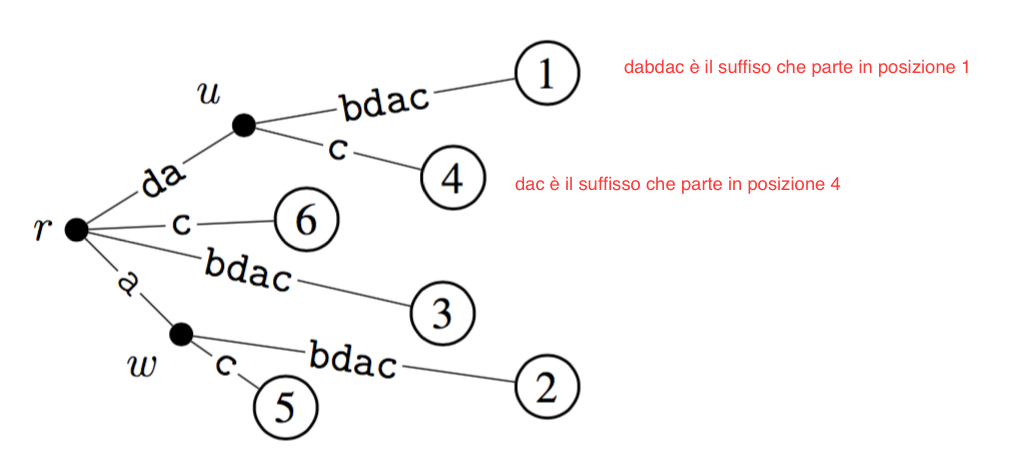
\includegraphics[width=.7\textwidth]{./notes/immagini/l19-fig1.png}
\caption{Albero dei suffissi della stringa $ S = dabdac $}
\end{figure}

Da notare che non sempre è possibile costruire l'albero dei suffusi, perché se un suffisso è anche prefisso di un altro suffisso, il cammino relativo a quel suffisso termina in un nodo interno dell'albero, violandone la definizione. 
Per evitare questo problema è necessario aggiungere un carattere sentinella alla fine della stringa. Assumeremo che questa ci sia sempre.

Nell'esempio \emph{S=dabdac} è \emph{c} che fa da sentinella, se non ci fosse non sarebbe possibile costruire l'albero.

L'\textbf{etichetta di un cammino} è la concatenazione delle etichette degli archi del cammino, mentre l'etichetta di un nodo \emph{u} è data dall'etichetta del cammino dalla radice al nodo.

Se l'etichetta di un arco $ (u,v) $ tra due nodi interni ha lunghezza \textit{k} maggiore di 1, l'arco è in realtà diviso in \textit{k} parti, una per ogni carattere dell'etichetta, mediante $ k-1 $ \textbf{nodi impliciti} le cui etichette sono la concatenazione dell'etichetta di \textit{u} con i caratteri dell'etichetta dell'arco $ (u,v) $ che precedono il nodo stesso.

\subsection{Matching esatto con l'albero dei suffissi}\label{matching-esatto-con-lalbero-dei-suffissi}

\begin{enumerate}
	\item Costruisci l'albero dei suffissi \textit{A} per il testo \textit{T}.
	\item Confronta i caratteri del pattern \textit{P} con i caratteri dell'unico cammino in \textit{A} individuato da essi. Questo cammino è unico perché tutti gli archi uscenti di un nodo sono associati a caratteri distinti. Seguendo questo cammino si possono verificare due casi:
	\begin{enumerate}
		\item Si esauriscono i caratteri del pattern e si passa al passo successivo
		\item Ci sono ancora dei caratteri del pattern ma non è possibile proseguire il cammino, in questo caso non ci sono occorrenze del pattern nel testo e l'algoritmo può terminare.
	\end{enumerate}
	\item Se si arriva alla fine del pattern, allora questo è uguale all'etichetta del nodo \textit{u} a cui si è arrivati, indipendentemente dal fatto che \textit{u} sia un nodo implicito o meno. Il pattern \textit{P} è quindi prefisso di tutti i suffissi associati alle foglie del sotto-albero radicato in \textit{u}. Le posizioni d'inizio di questi suffissi sono quindi tutte e sole le posizioni in cui \textit{P} occorre in \textit{T} e dal momento che queste posizioni sono memorizzate nelle foglie del sotto-albero, è sufficiente esplorarlo fino alle foglie per risalire alle posizioni di occorrenza del pattern.
\end{enumerate}

\subsubsection{Complessità del matching esatto}\label{complessituxe0-del-matching-esatto}

C'è una complessità \emph{O(n)} per la costruzione dell'albero (che per il momento non è stata vista).

Durante il secondo passo, per ogni carattere del pattern viene fatto
\begin{itemize}
	\item Un confronto se l'algoritmo sta analizzando un nodo implicito (c'è un solo arco uscente)
	\item Al più tanti confronti quanti sono i caratteri dell'alfabeto se è un nodo esplicito (al massimo ci sono tanti archi uscenti quanti sono i caratteri dell'alfabeto).
\end{itemize}

In ogni caso il numero di confronti è minore o uguale di una costante e quindi il passo 2 ha complessità $ O(m) $.

Il terzo passo richiede tempo proporzionale al numero di nodi del sotto-albero radicato in \textit{u}.
Se nel testo ci sono \textit{k} occorrenze del pattern, questo sotto-albero ha esattamente \textit{k} foglie e siccome ogni nodo interno ha almeno due archi uscenti, il numero di nodi interni è $ \leq k-1 $, quindi il terzo passo richiede $ O(k) $.

Siccome $ k \leq n $, il tempo totale richiesto è $ O(n+m) $, come per gli altri algoritmi, con la differenza che il carico di lavoro è sbilanciato verso la preelaborazione e non verso la ricerca (risulta più conveniente cercare più pattern nello stesso testo).

\subsection{L'algoritmo naive per la costruzione dell'albero} \label{lalgoritmo-naive-per-la-costruzione-dellalbero}

L'albero dei suffissi per la stringa $S[1,n]$ viene costruito a partire dal suffisso più lungo della stringa \textit{S}, ovvero tutta la stringa, per poi aggiungere gli altri suffissi $S[i,n]$ con $i = 2, \ldots, n+1$. 

Con $A_i$ viene indicato l'albero intermedio che contiene tutti i suffissi che iniziano nelle posizioni da 1 a \emph{i}.

L'albero $A_1$ contiene solamente un unico arco etichettato con $S[1,n]\$$ che congiunge la radice e il nodo \emph{1}.

Ogni albero $A_{i+1}$ viene costruito nel seguente modo:

\begin{enumerate}
	\item Partendo dalla radice di $ A_i $ viene cercato il più lungo cammino che raggiunge un nodo la cui etichetta è prefisso del suffisso $ S[i+1,n]\$ $ da aggiungere.
	
	Il cammino che si ottiene è unico in quanto ogni nodo implicito ha un solo arco uscente e tutti gli archi uscenti da uno stesso nodo esplicito sono associati a caratteri diversi.
	Inoltre, la ricerca deve terminare prima della fine del suffisso $ S[i+1,n]\$ $ perché la sentinella assicura che il suffisso non sia prefisso di nessuno dei prefissi più lunghi inseriti precedentemente nell'albero.
	
	\item Se il nodo in cui termina la ricerca è implicito, questo viene sostituito da un nodo esplicito, spezzando l'arco che lo contiene in due archi e l'etichetta in due etichette.
	
	\item A questo punto il nodo \textit{u} sul quale è terminata la ricerca è un nodo esplicito con etichetta $ S[i+1,j] $ tale che nell'albero non ci sia un nodo con etichetta $ S[i+1,j+1] $ e quindi tutti gli archi uscenti hanno etichette che iniziano con un carattere diverso da $ S[j+1] $.
	
	Viene quindi aggiunto un nuovo arco uscente da \textit{u} a $ i+1 $ con etichetta $ S[j+1,n]\$ $ che congiunge \textit{u} con la foglia numerata $ i+1 $.
	
	A questo punto l'albero ottenuto contiene un unico cammino dalla radice alla foglia $ i+1 $ la cui etichetta è il suffisso $ S[i+1,n]\$ $, ovvero l'albero ottenuto è $ A_{i+1} $
\end{enumerate}

\subsubsection{Complessità dell'algoritmo}\label{complessituxe0-dellalgoritmo}

Quando devo aggiungere un suffisso vengono passati al più tutti caratteri del suffisso e non appena viene trovato un carattere diverso, vengono aggiunti tanti nodi quanti sono i caratteri del suffisso restanti, ottenendo così una complessità $ O(n) $.
Dal momento che una stringa di lunghezza \textit{n} ha \textit{n} suffissi distinti, la complessità totale dell'algoritmo è $ O(n^2) $, dove $ n^2 $ è moltiplicato per una costante pari alla cardinalità dell'alfabeto.

\subsection{Algoritmo di Ukkonen}\label{algoritmo-di-ukkonen}

Questo algoritmo costruisce l'albero dei suffissi un carattere alla volta, partendo dall'inizio della stringa.

Così facendo viene persa la condizione che un suffisso non possa essere un prefisso dell'albero, per questo si dice che l'algoritmo crea una successione di \textbf{alberi dei suffissi impliciti}.

Un albero dei suffissi implicito è un albero simile a quello normale, con la differenza che viene rimossa la condizione che il cammino relativo ad ogni suffisso della stringa \textit{S} termini in una foglia e viene preso in considerazione anche il suffisso nullo.

\begin{figure}[htbp]
	\centering
	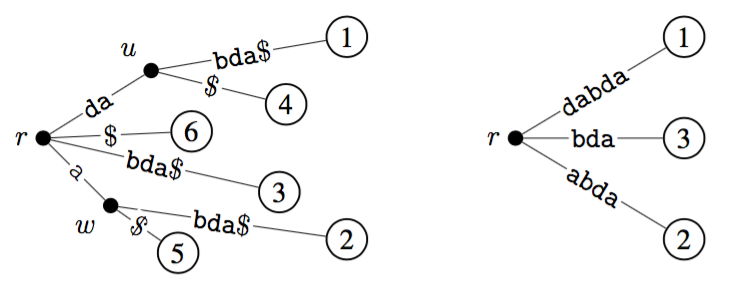
\includegraphics[width=.7\textwidth]{./notes/immagini/l19-fig2.png}
	\caption{Albero dei suffissi normale e implicito per la stringa $ S = dabda $.}
\end{figure}

L'algoritmo di Ukkonen costruisce un albero dei suffissi implicito $ I_i $ per ogni prefisso $ S[1,i] $ della stringa $ S\$ $ di lunghezza $ n+1 $ e incrementando \textit{i} finché non arriva a costruire $ I_{n+1} $. Siccome $ S[1,n+1] = S\$ $, l'albero dei suffissi implicito $ I_{n+1} $ coincide con l'albero dei suffissi \textit{A}, perché nessun suffisso della strina $ S\$ $ è prefisso di un altro suffisso.

\begin{breakablealgorithm}
	\caption{Ukkonen: Descrizione generale dell'algoritmo }
	\begin{algorithmic}[1]
		\Function{Ukkonen}{$S$}
			\State $ S \gets S\$ $ \Comment{Aggiunge la sentinella a $ S $}
			\State ``Costruisci $ I_0 $ ''
			\For{$ i = 0 \textbf{ to } n $}
				\For{$ j = 1 \textbf{ to } i+1 $}
					\State ``Cerca la fine del cammino relativo al suffisso $ S[j,i] $ in $ I_i $''
					\State ``Se necessario estendi il cammino con il carattere $S[i+1] $ in modo che il suffisso $ S[j,i] $ diventi un suffisso di $ S[1,i+1] $''
				\EndFor
			\EndFor
		\EndFunction
	\end{algorithmic}
\end{breakablealgorithm}

La costruzione di $ I_0 $ è banale in quanto contiene solo la radice e nessun arco uscente, perché la stringa $ S[1,0] $ ha come suffisso solamente $ \epsilon $.

Per costruire $ I_{i+1} $ è necessario modificare tutti i suffissi $ S[j,i] $ di $ S[1,i] $ nei suffissi $ S[j,i+1] $ di $ S[1,i+1] $.
Durante questa modifica possono verificarsi 3 casi:

\begin{enumerate}
	\item Il cammino etichettato $ S[j,i] $ termina in una foglia numerata $ j $. In questo caso il nuovo carattere $ S[i+1] $ viene aggiunto all'etichetta dell'ultimo arco del cammino (viene messo un nuovo nodo implicito).
	\item Il cammino etichettato $ S[j,i] $ termina in nodo interno \textit{u}, ma nessun cammino che parte da \textit{u} inizia con $ S[i+1] $. In questo caso viene creata una foglia etichettata $ j $ connessa al nodo \textit{u} con un arco etichettato $ S[i+1] $. Se \textit{u} è un nodo implicito, viene sostituito con un nodo esplicito, spezzando l'arco esistente.
	\item Il cammino etichettato $ S[j,i] $ termina in nodo interno \textit{u} e almeno un cammino che parte da \textit{u} è etichettato con $ S[i+1] $. In questo caso il suffisso $ S[j,i+1] $ è già presente nell'albero e non occorre fare niente.
\end{enumerate}

Dopo aver esteso tutti i suffissi di $ S[1,i] $ l'albero contiene tutti i suffissi di $ S[1,i+1] $, compreso il suffisso nullo che è sempre rappresentato.

\begin{figure}[htbp]
	\centering
	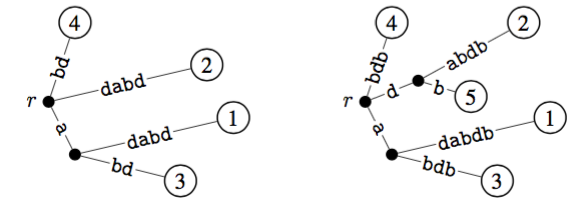
\includegraphics[width=.7\textwidth]{./notes/immagini/l19-fig3.png}
	\caption{Estensione dell'albero dei suffissi implicito per la stringa $ adabd $ quando si aggiunge alla stringa il carattere $ b $. I primi 4 suffissi vengono estesi con il caso 1, il quinto viene esteso con il caso 2 e il suffisso nullo viene esteso per il caso 3.}
\end{figure}

Tuttavia con questa implementazione si riesce a calcolare in $ O(i^2) $ l'albero $ I_{i+1} $ a partire da $ I_i $, portando ad una complessità totale di $ O(n^3) $ che è peggiore di quella dell'algoritmo naive.
